% Document setup
\documentclass[12pt]{article}
\usepackage[margin=1in]{geometry}
\usepackage{fancyhdr}
\usepackage{lastpage}

\pagestyle{fancy}
\lhead{Richard Whitehill}
\chead{PHYS 804 -- HW \HWnum}
\rhead{\duedate}
\cfoot{\thepage \hspace{1pt} of \pageref{LastPage}}

% Encoding
\usepackage[utf8]{inputenc}
\usepackage[T1]{fontenc}

% Math/Physics Packages
\usepackage{amsmath}
\usepackage{amssymb}
\usepackage{mathtools}
\usepackage{physics}
\usepackage{siunitx}

\AtBeginDocument{\RenewCommandCopy\qty\SI}

% Enumeration/itemize
\usepackage{enumitem}
\newenvironment{parts}
{\begin{enumerate}[label=\textbf{(\alph*)},leftmargin=*,itemsep=-10pt]
}{\end{enumerate}}

% Reference Style
\usepackage{hyperref}
\hypersetup{
    colorlinks=true,
    linkcolor=blue,
    filecolor=magenta,
    urlcolor=cyan,
    citecolor=green
}

\newcommand{\eref}[1]{Eq.~(\ref{eq:#1})}
\newcommand{\erefs}[2]{Eqs.~(\ref{eq:#1})--(\ref{eq:#2})}

\newcommand{\fref}[1]{Fig.~\ref{fig:#1}}
\newcommand{\frefs}[2]{Figs.~\ref{fig:#1}--\ref{fig:#2}}

\newcommand{\tref}[1]{Table~\ref{tab:#1}}
\newcommand{\trefs}[2]{Tables~\ref{tab:#1}-\ref{tab:#2}}

% Figures and Tables 
\usepackage{graphicx}
\usepackage{float}
\usepackage[font=small,labelfont=bf]{caption}

\newcommand{\bef}{\begin{figure}[h!]\begin{center}}
\newcommand{\eef}{\end{center}\end{figure}}

\newcommand{\bet}{\begin{table}[h!]\begin{center}}
\newcommand{\eet}{\end{center}\end{table}}

% tikz
\usepackage{tikz}
\usetikzlibrary{calc}
\usetikzlibrary{decorations.pathmorphing}
\usetikzlibrary{decorations.markings}
\usetikzlibrary{arrows.meta}
\usetikzlibrary{positioning}
\usetikzlibrary{3d}
\usetikzlibrary{shapes.geometric}

% tcolorbox
\usepackage[most]{tcolorbox}
\usepackage{xcolor}
\usepackage{xifthen}
\usepackage{parskip}

\newcommand*{\eqbox}{\tcboxmath[
    enhanced,
    colback=black!10!white,
    colframe=black,
    sharp corners,
    size=fbox,
    boxsep=8pt,
    boxrule=1pt
]}

% problem-solution macros
% \usepackage{adjustbox}
\usepackage{changepage}

\newtcolorbox{probbox}[1][]{
    breakable,
    enhanced,
    boxrule=0pt,
    frame hidden,
    borderline west={4pt}{0pt}{green!50!black},
    colback=green!5,
    before upper=\textbf{Problem #1) \,},
    % \textbf{Problem #1 \ifthenelse{\isempty{#1}}{}{: #1} \\ },
    sharp corners,
    parbox=false
}

% \newtcolorbox{ProblemBox}[1][]{%
%   breakable,
%   enhanced,
%   colback=black!10!white,
%   colframe=black,
%   title={\large #1 \hfill}
% }
\newcommand{\prob}[2]{
\begin{probbox}[#1]
#2
\end{probbox}
}

\newenvironment{solution}{\begin{adjustwidth}{8pt}{8pt}}{\end{adjustwidth}}
\newcommand{\sol}[1]{
\begin{solution}
#1
\end{solution}
}
% \textbf{#1)} #2}

% Miscellaneous Definitions/Settings
\newcommand{\reals}{\mathbb{R}}
\newcommand{\integers}{\mathbb{Z}}
\newcommand{\naturals}{\mathbb{N}}
\newcommand{\rationals}{\mathbb{Q}}
\newcommand{\complexs}{\mathbb{C}}

\setlength{\parskip}{\baselineskip}
\setlength{\parindent}{0pt}
\setlength{\headheight}{14.49998pt}
\addtolength{\topmargin}{-2.49998pt}


\def\HWnum{Final Project}
\def\duedate{December 9, 2024}


\begin{document}

\section{Introduction}
\label{sec:introduction}

Scattering is one of the most productive methods used to date to learn about the structure and contents of our universe.
In a previous project this semester, we studied scattering from a central force field in a classical context by numerically integrating the ordinary differential equations of motion provided by Newton's $2^{\rm nd}$ law.
While Rutherford scattering is quite a robust problem, generating the same results in classical mechanics and Born level in quantum mechanics, realistically speaking, we should handle such systems quantum mechanically.
In this article, we make a first pass at studying scattering in a quantum mechanical regime, restricting our attention to only one dimension.

The remainder of this article is organized as follows.
In Sec. \ref{sec:mathematical-framework}, we set up the problem to be studied, remind ourselves of the analytic methods used to broach the problem, and finally detail the numerical techniques we will use to solve the problem numerically.
Next, in Sec. \ref{sec:numerical-simulations}, we apply our numerical schemes to some analytically solvable cases and discuss the performance of our numerical solutions.
Finally, in Sec. \ref{sec:conclusions}, we summarize our findings and remark on future work to improve them and extend toward a full three dimensional scattering framework.


\section{Mathematical framework}
\label{sec:mathematical-framework}


\subsection{Setting up the problem}

Our problem of interest in this article is one dimensional scattering in non-relativistic quantum mechanics.
As with all non-relativistic quantum mechanical problems, the fundamental equation governing all dynamics is the Schr\"{o}dinger equation\footnote{Note that we work in natural units where $\hbar = c = 1$. This implies that the time and spatial dimensions are equivalent as well as the energy, momentum, and mass dimansions. Additionally, in this system of units, the spatial and energy dimensions are inverses of each other, which allows us to remain agnostic regarding the exact scales of our problem.}
\begin{align}
\label{eq:td-S-eq}
    i \pdv{\Psi(x,t)}{t} = -\frac{1}{2m} \dv[2]{\Psi(x,t)}{x} + V(x) \Psi(x,t)
.\end{align}
The typical analytic method for solving these problems is to separate the temporal and spatial dependence as $\Psi_{E}(x,t) = e^{- i E t} \psi_{E}(x)$, where the stationary solution $\psi_{E}(x)$ satisfies the time-independent Schr\"{o}dinger equation with corresponding energy eigenvalue $E$:
\begin{align}
\label{eq:ti-S-eq}
    -\frac{1}{2m} \dv[2]{\psi_{E}}{x} + V(x) \psi_{E} = E \psi_{E}
.\end{align}
Because this is a Sturm-Liouville problem, the separable solutions are complete in our domain of interest, allowing us to expand any wave-function of interest in these separable solutions:
\begin{align}
\label{eq:psi-expansion}
    \Psi(x,t) = \sum_{E} c(E) e^{-i E t} \psi_{E}(x)
,\end{align}
where $|c(E)|^2$ denotes the relative contribution of a particular stationary state in the spectrum of our system to our wave function.
As a further remark, note that for this article, because we are interested in scattering, we will only include the so-called scattering states with $E > \lim_{|x| \rightarrow \infty} V(x)$ such that there is no contamination from bound states.
To this end, for the rest of our analytic treatment, we assume that our potential is localized such that $\lim_{|x| \rightarrow \infty} V(x) = 0$.
In this asymptotic region, we can treat our particle as free and describe it as a wave packet, constructd from plane waves $\psi_{k}(x) = e^{i k x}$ with $E = k^2 / 2m$.

\subsection{Wave packet treatment}
\label{ssec:wave-packet-treatment}

In order to understand the treatment of wave packets, we consider the case of a $\delta$-function potential given by $V(x) = V_0 \delta(x)$, which although not quite physical illustrates clearly without much technical difficulty.
Clearly, the asymptotic regions are just $x < 0$ and $x > 0$, where our particle has momentum $\pm k$.
Although the eigenvalue $E = k^2/2m$ is doubly degenrate then, we choose the one corresponding to, as will become clear, an incident particle traveling from left to right and therefore $k > 0$ such that
\begin{align}
    \psi_{k}(x) = 
    \begin{cases}
        e^{i k x} + A(k) e^{-i k x} & x < 0 \\
        B(k) e^{i k x} & x > 0
    .\end{cases}
\end{align}
For our boundary conditions, we have $\psi_{k}(0^{-}) = \psi_{k}(0^{+})$ and $\psi_{k}'(0^{+}) - \psi_{k}'(0^{-}) = 2 m V_0 \psi_{k}'(0)$, which constrain our coefficients to be
\begin{align}
    A(k) &= -\frac{i V_0 m}{k + i V_0 m} \\
    B(k) &= \frac{k}{k + i V_0 m}
.\end{align}
We can then construct a wave-packet for all times $t$ by summing these energy eigenstates as follows:
\begin{align}
    \Psi(x,t) &= \int_{0}^{\infty} \frac{\dd{k}}{\sqrt{2 \pi}} g(k) \psi_{k}(x) \nonumber \\
              &= \Theta(-x) \Bigg\{ \int_{0}^{\infty} \frac{\dd{k}}{\sqrt{2 \pi}} g(k) e^{i k x - i k^2 t / (2m)} + \int_{0}^{\infty} \frac{\dd{k}}{\sqrt{2 \pi}} g(k) A(k) e^{-i k x - i k^2 t / (2m)} \Bigg\} \nonumber \\
              &+ \Theta(x) \int_{0}^{\infty} \frac{\dd{k}}{\sqrt{2 \pi}} g(k) B(k) e^{i k x - i k^2 t / (2m)}
,\end{align}
where $g(k)$ is some properly chosen real profile function.

We are now interested in understanding how the wave packet will appear after scattering from the potential.
The analysis is made more tractable and cleaner if our wave packets have momentum modes sharply centered at some $k = k_0$.
Making this assumption, we proceed via the method of stationary phase.
Let us analyze the form of each term separately, beginning with the incident wave packet
\begin{align}
    \Psi_{I}(x,t) = \int_{0}^{\infty} \frac{\dd{k}}{\sqrt{2 \pi}} g(k) e^{i \varphi_{I}(x,t,k)}
,\end{align}
where $\varphi_{I}(x,t,k) = kx - k^2 t / 2m$.
Since $g(k)$ is sharply peaked around some $k_0$, we expand the phase function about $k_{0}$ as
\begin{align}
    \varphi_{I}(x,t,k) &= \varphi_{I}(x,t,k_0) + (k - k_0) \dv{\varphi_{I}}{x}\Big|_{k=k_0} + \mathcal{O}\Big( (k - k_0)^2 \Big) \nonumber \\
                       &\approx \varphi_{I}(x,t,k_0) + (k - k_0) (x - x_{i}(t))
,\end{align}
where $x_{I}(t) = k_0 t / m$ satisfies $\dv*{\varphi_{I}}{k}|_{k=k_0,x=x_{I}(t)} = 0$ and is representative of the center of our incoming wave packet and corresponds approximately to the position of our wave packet with stationary phase, which is the inspiration for the method's name.
Using this, we write
\begin{align}
    \Psi_{I}(x,t) \approx e^{i \varphi_{I}(x,t,k_{0})} \int_{0}^{\infty} \frac{\dd{k}}{\sqrt{2 \pi}} g(k) e^{i (k - k_0) (x - x_{I}(t))}
.\end{align}
Observe that since $g(k)$ is sharply peaked around $k = k_0 > 0$, it is inconsequential to extend the integration range to all $k$ as
\begin{align}
    \Psi_{I}(x,t) &\approx e^{i \varphi_{I}(x,t,k_0)} \int_{-\infty}^{\infty} \frac{\dd{k}}{\sqrt{2 \pi}} g(k) e^{i (k - k_0) (x - x_{I}(t))} \nonumber \\
                  &= e^{i [ \varphi_{I}(x,t,k_0) - k_0 (x - x_{I}(t)) ]} \int \frac{\dd{k}}{\sqrt{2 \pi}} g(k) e^{i k ( x - x_{I}(t) )} \nonumber \\
                  &= e^{i[\varphi_{I}(x,t,k_0) - k_0 (x - x_{I}(t))]} G(x - x_{I}(t))
,\end{align}
where $G(x)$ is the inverse Fourier transform of $g(k)$.
Next, we analyze the form of the reflected wave packet.
Defining $A(k) = |A(k)| e^{-i \chi_{A}(k)}$ such that
\begin{align}
    |A(k)| = \frac{V_0^2 m^2}{k^2 + V_0^2 m^2}~{\rm and}~\tan{\chi_{A}(k)} = -\frac{k}{m V_0}
,\end{align}
we write
\begin{align}
    \Psi_{R}(x,t) = \int_{0}^{\infty} \frac{\dd{k}}{\sqrt{2 \pi}} g(k) |A(k)| e^{-i \varphi_{R}(k)}
,\end{align}
so that the overall reflected phase function
\begin{align}
    \varphi_{R}(x,t,k) = kx + \frac{k^2 t}{2m} + \chi_{A}(k)
.\end{align}
Performing the stationary phase expansion, we find
\begin{align}
    \varphi_{R}(x,t,k) \approx \varphi_{R}(x,t,k_0) + (k - k_0) (x - x_{R}(t))
,\end{align}
where 
\begin{align}
    x_{R}(t) &= - \frac{k_0 t}{m} - \chi_{r}'(k_0) = -\frac{k_0 t}{m} + \frac{1}{m V_0} \frac{1}{1 + {\rm arctan}^2(k_0 / m V_0)} \nonumber \\
    &= -\frac{k_0}{m} \Bigg\{ t - \frac{1}{k_0 V_0} \frac{1}{1 + \arctan^2(k_0/m V_0)} \Bigg\}
.\end{align}
With this, we have
\begin{align}
    \Psi_{R}(x,t) = |A(k_0)| e^{i [ \varphi_{R}(x,t,k_0) - k_0(x - x_{R}(t)) ]} G(x - x_{R}(t))
.\end{align}
Similarly, for the transmitted wave packet
\begin{align}
    \Psi_{T}(x,t) &= \int_{0}^{\infty} \frac{\dd{k}}{\sqrt{2 \pi}} g(k) |B(k)| e^{i \varphi_{T}(x,t,k)}
\end{align}
with $\varphi_{T}(x,t,k) = k x - k^2 t / (2m) - \chi_{B}(k)$ so that
\begin{align}
    x_{T}(t) = \frac{k_0 t}{m} + \chi_{B}'(k) = \frac{k_0}{m} \Bigg\{ t - \frac{m^2 V_0}{k_0^3} \frac{1}{1 + \arctan^2(m V_0 / k_0)} \Bigg\}
\end{align}
and
\begin{align}
    \Psi_{T}(x,t) = |B(k_0)| e^{i [ \varphi_{T}(x,t,k_0) - k_0 ( x - x_{T}(t) ) ]} G(x - x_{T}(t))
.\end{align}
With this, we have essentially concluded our analysis for scattering from a $\delta$-function potential with a wave packet moving with a nearly uniform momentum.

The upshot of all this work is the following.
When we prepare a wave packet with a very narrow momentum spectrum that is sent towards a localized momentum, then after a sufficient amount of time -- determined by the particle's mass and average momentum as well as the specifics of the potential -- we observe reflected and transmitted wave packets in the asymptotic region with approximately the same shape as our incident wave packet, modulated by some transmission and reflection amplitudes that obey probability conservation as
\begin{align}
    |A(k_0)|^2 + |B(k_0)|^2 = 1
,\end{align}
which can be shown by considering the normalization of the wave function in the asymptotic limits $t \rightarrow \pm \infty$.
Thus, $|A(k)|^2$ gives us the probability for a wave packet with momentum $k$ to scatter backwards toward $x \rightarrow -\infty$ while $|B(k)|^2$ gives us the probability for a wave packet to be transmitted through the potential and propagate toward $x \rightarrow \infty$.

In this article, our goal will be to map out the these reflection and transmission probabilities.
To this end, for our numerical simulations, we will prepare wave packet states localized in momentum space far from some potential of interest, evolve our system in time until we have our reflected and transmitted wave packets in the asymptotic region, and finally compute the reflection and transmission probabilities as
\begin{align}
\begin{aligned} 
    |A(k)|^2 &= \lim_{t \rightarrow \infty} \int \dd{x} |\Psi_{R}(x,t)|^2 \\
    |B(k)|^2 &= \lim_{t \rightarrow \infty} \int \dd{x} |\Psi_{T}(x,t)|^2
.\end{aligned}
\end{align}


\subsection{Numerical techniques for unitary time evolution}
\label{ssec:numerical-techniques-for-unitary-time-evolution}

According to Eq. (\ref{eq:psi-expansion}), if we know the spectrum of our theory, then we can automatically expand our wave packet in the scattering states with the time evolution given by the factor $e^{-i E t}$.
In practice, though, it may not be such a simple matter or even possible to solve the time-independent Schr\"{o}dinger equation for a given potential in closed form.
We could perhaps adopt the same approach as in Project 3 where we discretized Eq. (\ref{eq:ti-S-eq}) to transform it into an eigenvalue problem.
However, unlike in the case where we were interested in solving for bound state wave functions and energies, in the case of scattering states, we know \textit{a priori} our energy eigenvalues for scattering states and further that our energy spectrum is continuous.
Therefore, it is somewhat problematic to only receive a finite number of energy eigenvalues which we cannot necessarily gurantee will be centered on any momentum mode or how densely the eigenvalues would be spaced.
Additionally, for bound states, it is natural to impose Dirichlet conditions since our solutions must vanish in the asymptotic regions, but for the localized potentials here, our solutions will be plane waves.
Although, our physical wave packet must vanish far from the center, the separable solutions do not.
Hence, it is not clear from the onset how to a more natural set of boundary conditions on our scattering state solutions.

Because of the difficulties layed out above, instead of solving the time-independent Schr\"{o}dinger equation and splicing together the stationary states as in Eq. (\ref{eq:psi-expansion}), we will solve the time-dependent Schr\"{o}dinger equation directly with the boundary condition at $t = 0$ given by an appropriate wave packet.
The first attempt made to simulate the time evolution of a wave packet utilized the finite difference method, discretizing our spatial and temporal domain to yield a transfer matrix $U$ which evolved our wave function from one time slice to the next.
However, in practice, we do not use this method for a few troublesome reasons.
Primarily, though, the transfer matrix $U$ violates unitarity at the order of $\Delta t^2$, where $\Delta t$ is the size of the time step, and while this is not an issue over only a few time steps, the errors propagate dramatically over a sizable number of steps, which implies that probability is not properly conserved.
For more details on this method, a derivation and discussion are placed in App. \ref{app:finite-differences}.

Finally, we come to the Fourier transform inspired method that we use in our simulations.
Instead of discretizing our wave packets from the onset and obtaining a finite transfer matrix $U$, we recall that we can introduce the unitary time evolution operator $U(t,t')$, which evolves our wave function at time $t'$ to time $t$ via $\Psi(x,t) = U(t,t') \Psi(x,t')$.
From this requirement, we deduce that $U$ satisfies the operator equation
\begin{align}
    i \pdv{U(t,t')}{t} = H U(t,t')
,\end{align}
which has solution
\begin{align}
    U(t,t') = e^{-i H (t - t')}
\end{align}
if $H$ is independent of time as will be the case in our scattering problems.
Let us write $H = H_0 + V$, where $H_0$ is the free-particle Hamiltonian and $V$ contains the potential terms.
If we select our time step $\Delta t$ between time slices $t_{m}$ and $t_{m+1}$, then using the Baker-Campbell-Hausdorff formula, we can write
\begin{align}
    U(\Delta t) &= e^{-i H \Delta t} = e^{-i H_0 \Delta t - i V \Delta t} \approx e^{-i H_0 \Delta t} e^{-i V \Delta t} e^{\frac{\Delta t^2}{2} [H_0, V]} \nonumber \\
                &= e^{-i H_0 \Delta t} e^{-i V \Delta t} \Big( 1 + \frac{\Delta t^2}{2} [H_0,V] + \mathcal{O}(\Delta t^{4}) \Big)
.\end{align}
For sufficiently small time steps, the free particle and potential pieces of the Hamiltonian can act separately on our wave packet, and because plane waves are eigenstates of the free particle Hamiltonian, we can express our wave function at the current time step $t_{m}$ as a Fourier transform and act the time evolution operator as follows:
\begin{align}
    \Psi(x,t_{m+1}) &= U(\Delta t) \Psi(x,t_{m}) = e^{-i V(x) \Delta t} \int \frac{\dd{k}}{\sqrt{2 \pi}} \widetilde{\Psi}(k,t_{m}) e^{-i H_0 \Delta t} e^{i k x} \nonumber \\
    &= e^{-i V(x) \Delta t} \int \frac{\dd{k}}{\sqrt{2 \pi}} \widetilde{\Psi}(k,t_{m}) e^{- i k^2 \Delta t / (2m)} e^{i k x}
,\end{align}
where $\widetilde{\Psi}(k,t_{m})$ is the Fourier transform of $\Psi(x,t_{m})$.
We see explicitly here that for small time steps, our potential changes the phase of the wave-function locally and the free part of the Hamiltonian propagates our modes according to the velocity $k/m$.

Because the above equation is set up on the continuous spatial domain we could set up our wave-packets as functions numerically and implement a numerical quadrature to take the Fourier transform at each $x$, but this could become quite computationally expensive both regarding resources and time.
We could, however, discretize our spatial domain and use the discrete Fourier transform (DFT), computed via the fast-fourier transform method.

We note that in practice, we cannot simply replace the CFT with a DFT and evaluate at the spatial grid points: we must include a few factors to correctly obtain the CFT from the DFT.
For brevity, consider some square integrable function $f(x)$.
The expressions we use for the continuous fourier and inverse fourier transforms of $f(x)$ are as follows:
\begin{align}
\begin{aligned} 
    f(x) &= \int \frac{\dd{k}}{\sqrt{2 \pi}} \tilde{f}(k) e^{i k x} \\
    \tilde{f}(k) &= \int \frac{\dd{x}}{\sqrt{2 \pi}} f(x) e^{-ikx}
.\end{aligned}
\end{align}
On the other hand, for a collection of discrete data points $f_{n}$, their discrete Fourier and inverse Fourier transforms are as follows (consistent with the \textit{numpy} conventions using the ``ortho'' normalization):
\begin{align}
\begin{aligned} 
    f_{n} &= \frac{1}{\sqrt{N}} \sum_{m=0}^{N-1} F_{m} e^{2 \pi i \frac{m n}{N}} \\
    F_{m} &= \frac{1}{\sqrt{N}} \sum_{n=0}^{N-1} f_{n} e^{-2 \pi i \frac{m n}{N}}
.\end{aligned}
\end{align}
We can write the grid points in $x$-space as $x_{n} = x_0 + n \Delta x$ and those in $k$-space as $k_{m} = m \Delta k$ with $n,m \in \{ 0,1,\ldots,N-1 \}$, where
\begin{align}
    \Delta x \Delta k = \frac{2 \pi}{N}
.\end{align}
From this discretization, we can approximate
\begin{align}
    \tilde{f}(k) = \sum_{n=0}^{N-1} \frac{\Delta x}{\sqrt{2 \pi}} f(x_{n}) e^{-i k x_{n}} = \frac{\Delta x \sqrt{N}}{\sqrt{2 \pi}} e^{-i k x_0} \frac{1}{\sqrt{N}} \sum_{n=0}^{N-1} f(x_{n}) e^{-i k n \Delta x}
.\end{align}
Hence,
\begin{align}
    \tilde{f}(k_{m}) = \frac{\Delta x \sqrt{N}}{\sqrt{2 \pi}} e^{-i k_{m} x_0} F_{m}
.\end{align}
We can also then perform the inverse fourier transform by writing $F_{m}$ in terms of $\tilde{f}(k_{m})$.

One thing to note with this method is that we have not imposed boundary conditions explicitly, but it can be seen that the Fourier method implicitly imposes periodic boundary conditions.
That is, any part of the wave packet which exits our physical numerical domain to the right appears back on the left part of our spatial domain and \textit{vice versa}.
To deal with this, we should ensure that our numerical domain is much larger than the extent of our potential such that our wave packets reach the asymptotic region before a significant portion of the transmitted or reflected wave packets enter the incorrect region of space and contribute to the wrong probability density.


\section{Numerical simulations}
\label{sec:numerical-simulations}

\subsection{Freely propagating Gaussian wave packet}
\label{ssec:freely-propagating-gaussian-wave-packet}

To test that our numerical solver works, we choose an initial wave function
\begin{align}
    \Psi(x,0) = \frac{1}{(2 \pi \sigma^2)^{1/4}} \exp{-\frac{(x - x_{0})^2}{4 \sigma^2}} \exp{i k x}
,\end{align}
which is a Gaussian density at $t = 0$ with average momentum $k$.
We can now use propagator formalism to determine the wave function at any later time $t$ as follows:
\begin{align}
\label{eq:gauss-wave-prop}
    \Psi(x,t) &= \int \dd{x'} K(x,x';t) \Psi(x',0) \nonumber \\
              &= \sqrt{\frac{m}{2 \pi i t}} \frac{1}{(2 \pi \sigma^2)^{1/4}} \int_{-\infty}^{\infty} \dd{x'} \exp{-\frac{m(x - x')^2}{2 i t} - \frac{(x' - x_0)^2}{4 \sigma^2} + i k x'}
.\end{align}
The intermediate form of the wave function is not too interesting for our purposes, but the probability density
\begin{align}
    |\Psi(x,t)|^2 = \frac{1}{\sqrt{2 \pi \sigma^2}} \frac{2 \sigma^2 m}{\sqrt{ 4 \sigma^4 m^2 + t^2 }} \exp{ -\frac{2 m^2 \sigma^2 [ x - (x_0 + k t / m) ]^2}{4 \sigma^{4} m^2 + t^2} }
.\end{align}


\begin{figure}[tb]
    \centering
    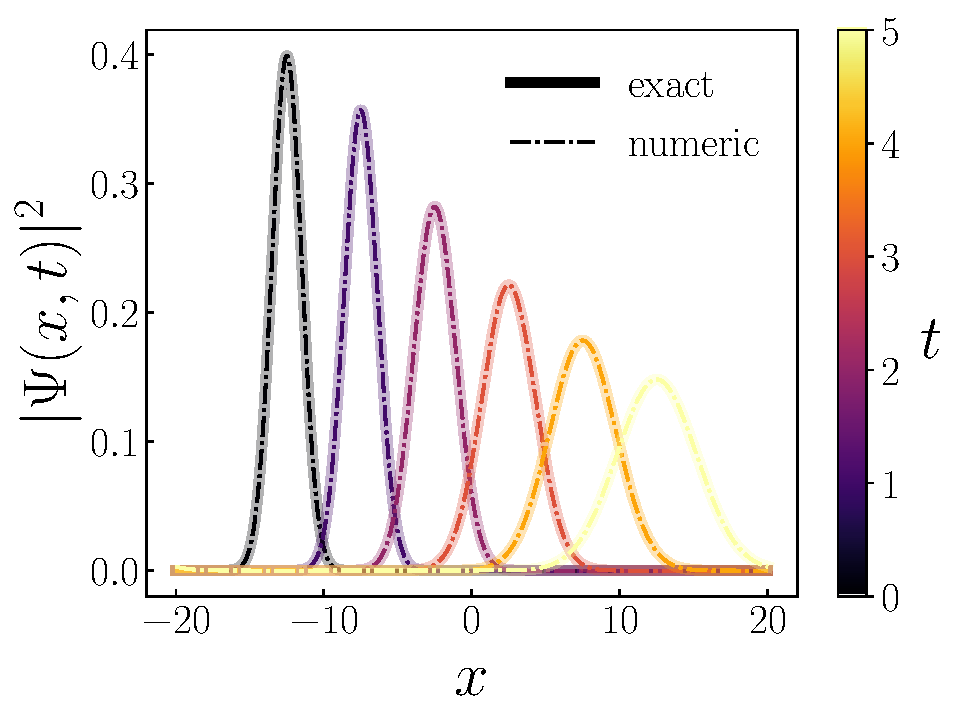
\includegraphics[width=0.7\linewidth]{gauss_wave-prop.pdf}
    \caption{Comparison of Gaussian wave-packet propagation, where the exact formula is given in Eq. \ref{eq:gauss-wave-prop}, with the numerical Fourier transform based numerical scheme presented in Sec. \ref{ssec:fourier-transform}.}
    \label{fig:gauss-wave-prop}
\end{figure}


\subsection{Square barrier}
\label{ssec:square-barrier}

For this section, we consider a potential of the form $V(x) = V_0 [ \Theta(x) - \Theta(x - a) ]$.
We then have two cases to consider.
First, if $E < V_0$, or equivalently $k < \sqrt{2 m V_0}$, we find
\begin{align}
    |A(k)| &= \frac{2 m V_0 \sinh(\kappa a)}{\sqrt{4 \kappa^2 k^2 + 4 m^2 V_0^2 \sinh^2(\kappa a)}} \\
    |B(k)| &= \frac{2 \kappa k}{\sqrt{4 \kappa^2 k^2 + 4 m^2 V_0^2 \sinh^2(\kappa a)}}
,\end{align}
where $\kappa = \sqrt{2 m V_0 - k^2}$.
Alternatively, if $E > V_0$, or equivalently $k > \sqrt{2 m V_0}$, we find
\begin{align}
    |A(k)| &= \frac{2 m V_0 |\sin(k' a)|}{\sqrt{4 k'^2 k^2 + 4 m^2 V_0^2 \sin^2(k' a)}} \\
    |B(k)| &= \frac{2 \kappa k}{\sqrt{4 k'^2 k^2 + 4 m^2 V_0^2 \sin^2(k' a)}}
,\end{align}
where $k' = \sqrt{k^2 - 2 m V_0}$.





\section{Conclusions}
\label{sec:conclusions}




\appendix

\section{Finite differences}
\label{app:finite-differences}

For our first numerical method, we solve the time-dependent Schr\"{o}dinger equation 
\begin{align}
    i \pdv{\Psi(x,t)}{t} = -\frac{1}{2m} \pdv[2]{\Psi(x,t)}{x} + V(x) \Psi(x,t)
.\end{align}
directly by implementing a finite difference scheme.
Using a forward difference formula for the time deriva, the three-point formula for the second derivative, and rearranging, we obtain
\begin{align}
    \Psi_{n}^{(m + 1)} = \Psi_{n}^{(m)} + i \Delta t \Bigg( \frac{\Psi_{n-1}^{(m)} - 2 \Psi_{n}^{(m)} + \Psi_{n+1}^{(m)}}{2m \Delta x^2} - V_{n} \Psi_{n}^{(m)} \Bigg)
,\end{align}
where $\Psi_{n}^{(m)} = \Psi(x_n,t_{m})$, $x_{n} = x_0 + n \Delta x$, and $t_{m} = m \Delta t$.
Thus, we have a sequence defined by $\Psi_{n}^{(m)} = U^{m} \Psi_{n}^{(0)}$, where
\begin{align}
    U_{kn} = \delta_{kn} - i \Delta t H_{kn}
,\end{align}
where the discretized Hamiltonian
\begin{align}
    H_{kn} = -\frac{\delta_{k-1,n} - 2 \delta_{kn} + \delta_{k+1,n}}{2m \Delta x^2} + V_{k} \delta_{kn}
.\end{align}
Such an equation reminds us of the unitary time evolution, which can be explored by direct matrix multiplication:
\begin{align}
    U_{kn}^{\dagger} U_{nk'} &= ( \delta_{kn} + i \Delta t H_{kn}^{\dagger} ) ( \delta_{nk'} - i \Delta t H_{nk'} ) = \delta_{k k'} + i \Delta t ( H_{kk'}^{\dagger} - H_{kk'} ) + \Delta t^2 H_{kn}^{\dagger} H_{nk'} \nonumber \\
    &= \delta_{kk'} + \mathcal{O}(\Delta t^2)
.\end{align}
Herein lies a primary difficulty of implementing this method: the eigenvalues of $U$ essentially scale the eigenvector components of our initial wavevector.
Hence, for stability, we would like to select $\Delta t$ and $\Delta x$ such that all of these eigenvalues are less than one.
Unfortunately, this is not possible since the eigenvalues of a unitary matrix have unit norm, prohibiting us from performing our time evolution in this manner.

{\color{red} 
    Make plots demonstrating instability.
}


\section{Stability of the explicit and implicit finite difference methods}
\label{app:stability-of-the-explicity-and-implicit-finite-difference-methods}

In this work, the operators we deal with are typically either hermitian or unitary, both of which are special cases of the broader class of normal matrices $A$ which commute with their hermitian conjugate $A^{\dagger}$.
There is a theorem of equivalence statements in linear algebra that defines a normal matrix and states that any normal matrix $A$ is diagonalizable via a unitary similarity transformation and that there exists a set of eigenvectors which forms an complete orthonormal basis for the $n$-dimensional vector space.
Let us denote the spectrum of $A$ by the set $\{ a_{n} \}$ and the corresponding set of eigenvectors by $\{ x^{(n)} \}$
Thus, any vector $\Psi$, which is analogous to our discretized wave-function, we can write
\begin{align}
    \Psi = \sum_{n} c_{n} x^{(n)}
,\end{align}
where $c_{n} = \Psi^{\dagger} x^{(n)}$.
It follows then, that repeated action of $A$ on $\Psi$ yields
\begin{align}
    \Psi^{(k)} = A^{k} \Psi = \sum_{n} c_{n} a_{n}^{k} x^{(n)}
.\end{align}
If we now consider $A$ to be nearly unitary, as in the finite difference methods above for time-evolution, then we see our fundamental issue with implementing the finite difference methods above.
Indeed, because of the discretization effects, our eigenvalues $a_{n}$ have approximately unit norm but not quite.
Thus, for large times (i.e. in the limit $k \rightarrow \infty$), we have
\begin{align}
    A^{k} \Psi \rightarrow c_{n_{\rm max}} a_{n_{\rm max}}^{k} x^{(n_{\rm max})}
,\end{align}
where $n_{\rm max} = {\rm argmax}(\{ a_{n} \})$.
Hence, if $a_{n_{\rm max}} > 1$, then our solution explodes, and if $a_{\rm max} < 1$, then our solution vanishes at large times.
Of course then, even the slightest bit of unitarity violation in our matrix evolution is a fatal flaw for a finite difference method propagating the entire wave-function, both its real and imaginary parts, at equal times.

    
\end{document}
